\section{Descripción detallada de casos de uso}

\subsection{Consultar precios de compra disponibles para un producto}

\textbf{Resumen:}
Dada una descripción o número de parte
-que es un nomenclador único de productos-,
el encargado de compras recibirá un listado de precios de dicho producto,
que será descargado de las páginas web e interfaces de programación de los diversos proveedores,
de acuerdo a disponibilidad.

\textbf{Precondición:} 
el encargado de compras ingresa parte del nombre/descripción/número de parte en el sistema para iniciar una búsqueda

\textbf{Escenario principal:}
\begin{enumerate}
	\item El encargado de compras ingresa a la opción búsqueda.
	\item El sistema solicita ingreso de número de parte, descripción o nombre, del producto.
	\item El encargado de compras ingresa cualquiera de los datos, de forma completa o parcial.
	\item El sistema muestra coincidencias al encargado de compras, para que elija cuál era el artículo buscado.
	\item El encargado de compras confirma el producto buscado.
	\item El sistema descarga la información necesaria, 
	recurriendo en los casos en que sea posible a las interfaces de programación de los proveedores (API),
	al \textit{Web Scrapping} donde no sea posible. Una vez recopilada la información, 
	se presenta al encargado por nombre de proveedor y precio.
	\item El encargado toma las decisiones correspondientes e inicia el proceso de compra por canales habituales.
\end{enumerate}

\textbf{Poscondición:}
El encargado de compras dispone de información suficiente, en tiempo real, para hacer una compra minimizando costos.

\textbf{Flujo alternativo:}

\textbf{A1} El nombre, descripción o número de parte no coincide con un producto cargado en base de datos.

La secuencia comienza en el punto 3.

\begin{enumerate}
	\item[4.] El sistema informa que no existen coincidencias con productos en base de datos,
	y solicita cargar número de parte íntegramente para buscar por nomenclador único.
	\item[5.] El usuario carga número de parte íntegramente.
	\item[6.] El sistema muestra coincidencias tomadas directamente de proveedor,
	de ser el producto buscado se incorpora a base de datos,
	para facilitar búsqueda por descripción o nombre en el futuro.
\end{enumerate}

El escenario vuelve a punto 6.

\textbf{A2} El nombre, descripción o número de parte no coincide con ningún producto, ni en base de datos ni en proveedor

La secuencia comienza en el punto 6 del flujo alternativo \textbf{A1}.

\begin{enumerate}
	\item [7.] El sistema informa que dicho número de parte no coincide con ningún producto en base de datos ni en proveedor y solicita corroborar dicho número o intentar nuevamente.
\end{enumerate}

El escenario vuelve al punto 2.

\begin{figure}[H]
	\centering
	\vspace{15pt}
	\caption{Caso de Uso 1 y Flujos Alternativos}
	\vspace{15pt}
	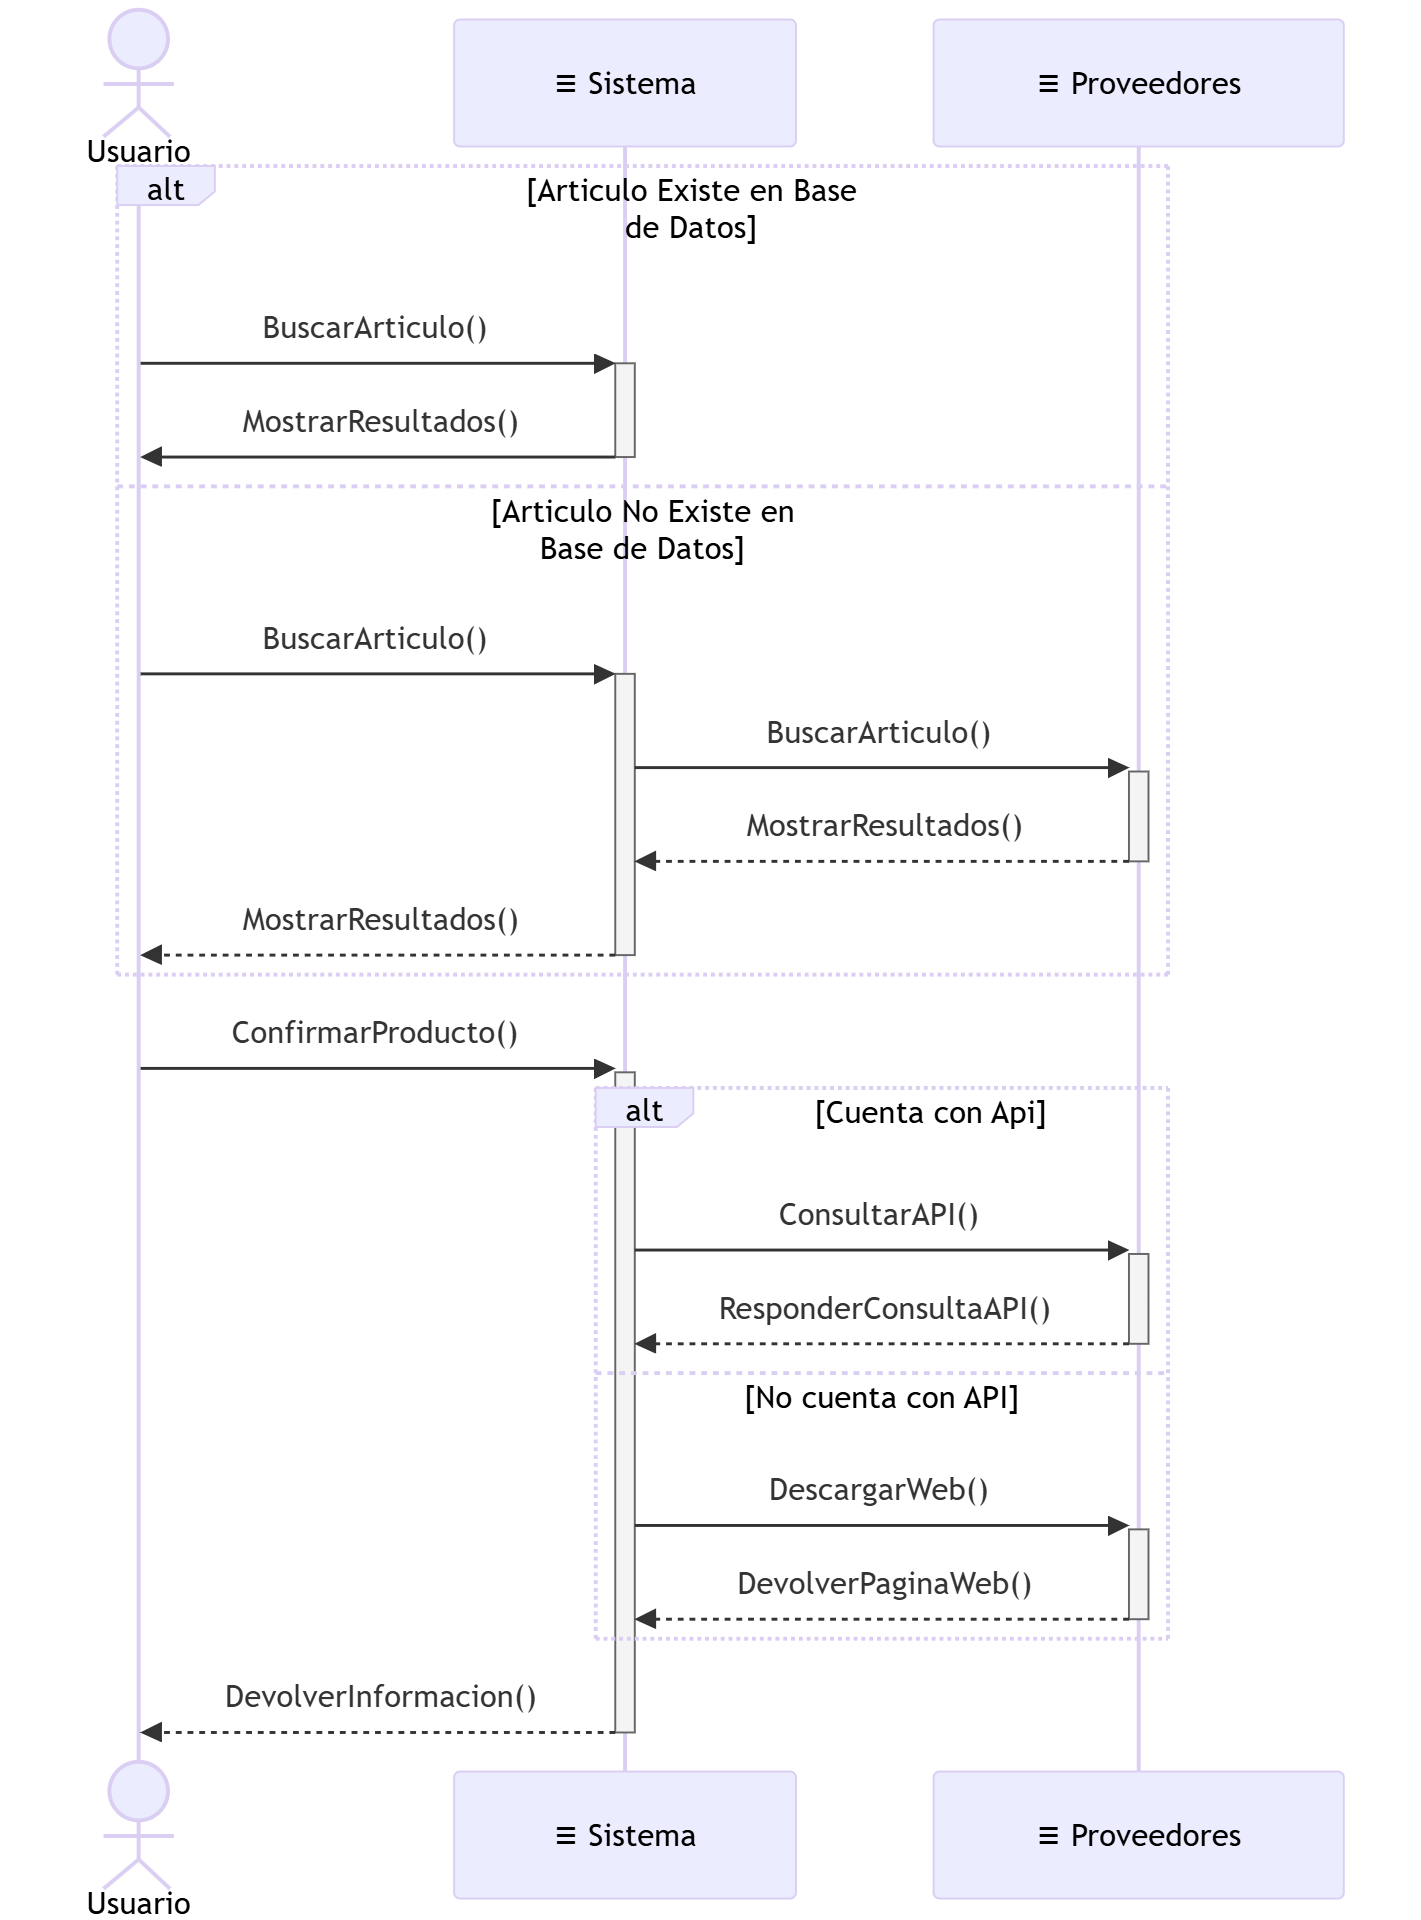
\includegraphics[width=.9\textwidth]{img/04-diagrama-caso-1.png}
	\vspace{15pt}
\end{figure}

\pagebreak

\subsection{Conocer los precios de la competencia}

\textbf{Resumen:}
Dado un número de parte, nombre, o descripción,
de forma íntegra o parcial,
el encargado de compras contará con un listado de precios de venta del producto,
que se descargará de páginas web y APIs de los portales de venta online,
de acuerdo a su disponibilidad.

\textbf{Precondición:} 
el encargado de compras ingresa -de manera parcial o completa- el nombre, descripción o número de parte de un producto

\textbf{Escenario principal:}
\begin{enumerate}
	\item El encargado de compras ingresa a la sección de búsqueda de \textbf{precios de venta}.
	\item El sistema solicita ingreso de número de parte, descripción o nombre del producto.
	\item El encargado de compras ingresa cualquiera de los datos, de forma completa o parcial.
	\item El sistema muestra coincidencias al encargado de compras, de manera tal que elija el artículo buscado.
	\item El encargado de compras confirma el producto buscado.
	\item El sistema descarga la información necesaria, 
	recurriendo de forma prioritaria a las interfaces de programación (API)
	y al \textit{Web Scrapping} donde no sea posible. Una vez recopilada la información, 
	se presenta al encargado incluyendo nombre de proveedor y precio.
	\item Contando con dicha información, más la suministrada de \textbf{precios de compra},
	el encargado de compras toma las decisiones correspondientes.
\end{enumerate}

\textbf{Poscondición:}
El encargado de compras dispone de información, 
en tiempo real, 
para detectar oportunidades de productos con costos relativamente bajos y precios de venta relativamente altos.

\textbf{Flujo alternativo:}

La secuencia comienza en el punto 3.

\begin{enumerate}
	\item[4.] El sistema informa que no existen coincidencias con productos en base de datos,
	y solicita cargar número de parte íntegramente para buscar por nomenclador único.
	\item[5.] El usuario carga número de parte íntegramente.
	\item[6.] El sistema muestra coincidencias tomadas directamente de portales de venta online,
	de ser el producto buscado se incorpora a base de datos,
	para facilitar búsqueda por descripción o nombre en el futuro.
\end{enumerate}

El escenario vuelve a punto 6.

\textbf{A2} El nombre, descripción o número de parte no coincide con ningún producto, ni en base de datos ni en portales de venta online de la competencia.

La secuencia comienza en el punto 6 del flujo alternativo \textbf{A1}.

\begin{enumerate}
	\item [7.] El sistema informa que dicho número de parte no coincide con ningún producto en base de datos ni en portales de venta online de la competencia, 
	solicita corroborar dicho número o intentar nuevamente más tarde.
\end{enumerate}

El escenario vuelve al punto 2.

\begin{figure}[H]
	\centering
	\vspace{15pt}
	\caption{Caso de Uso 2 y Flujos Alternativos}
	\vspace{15pt}
	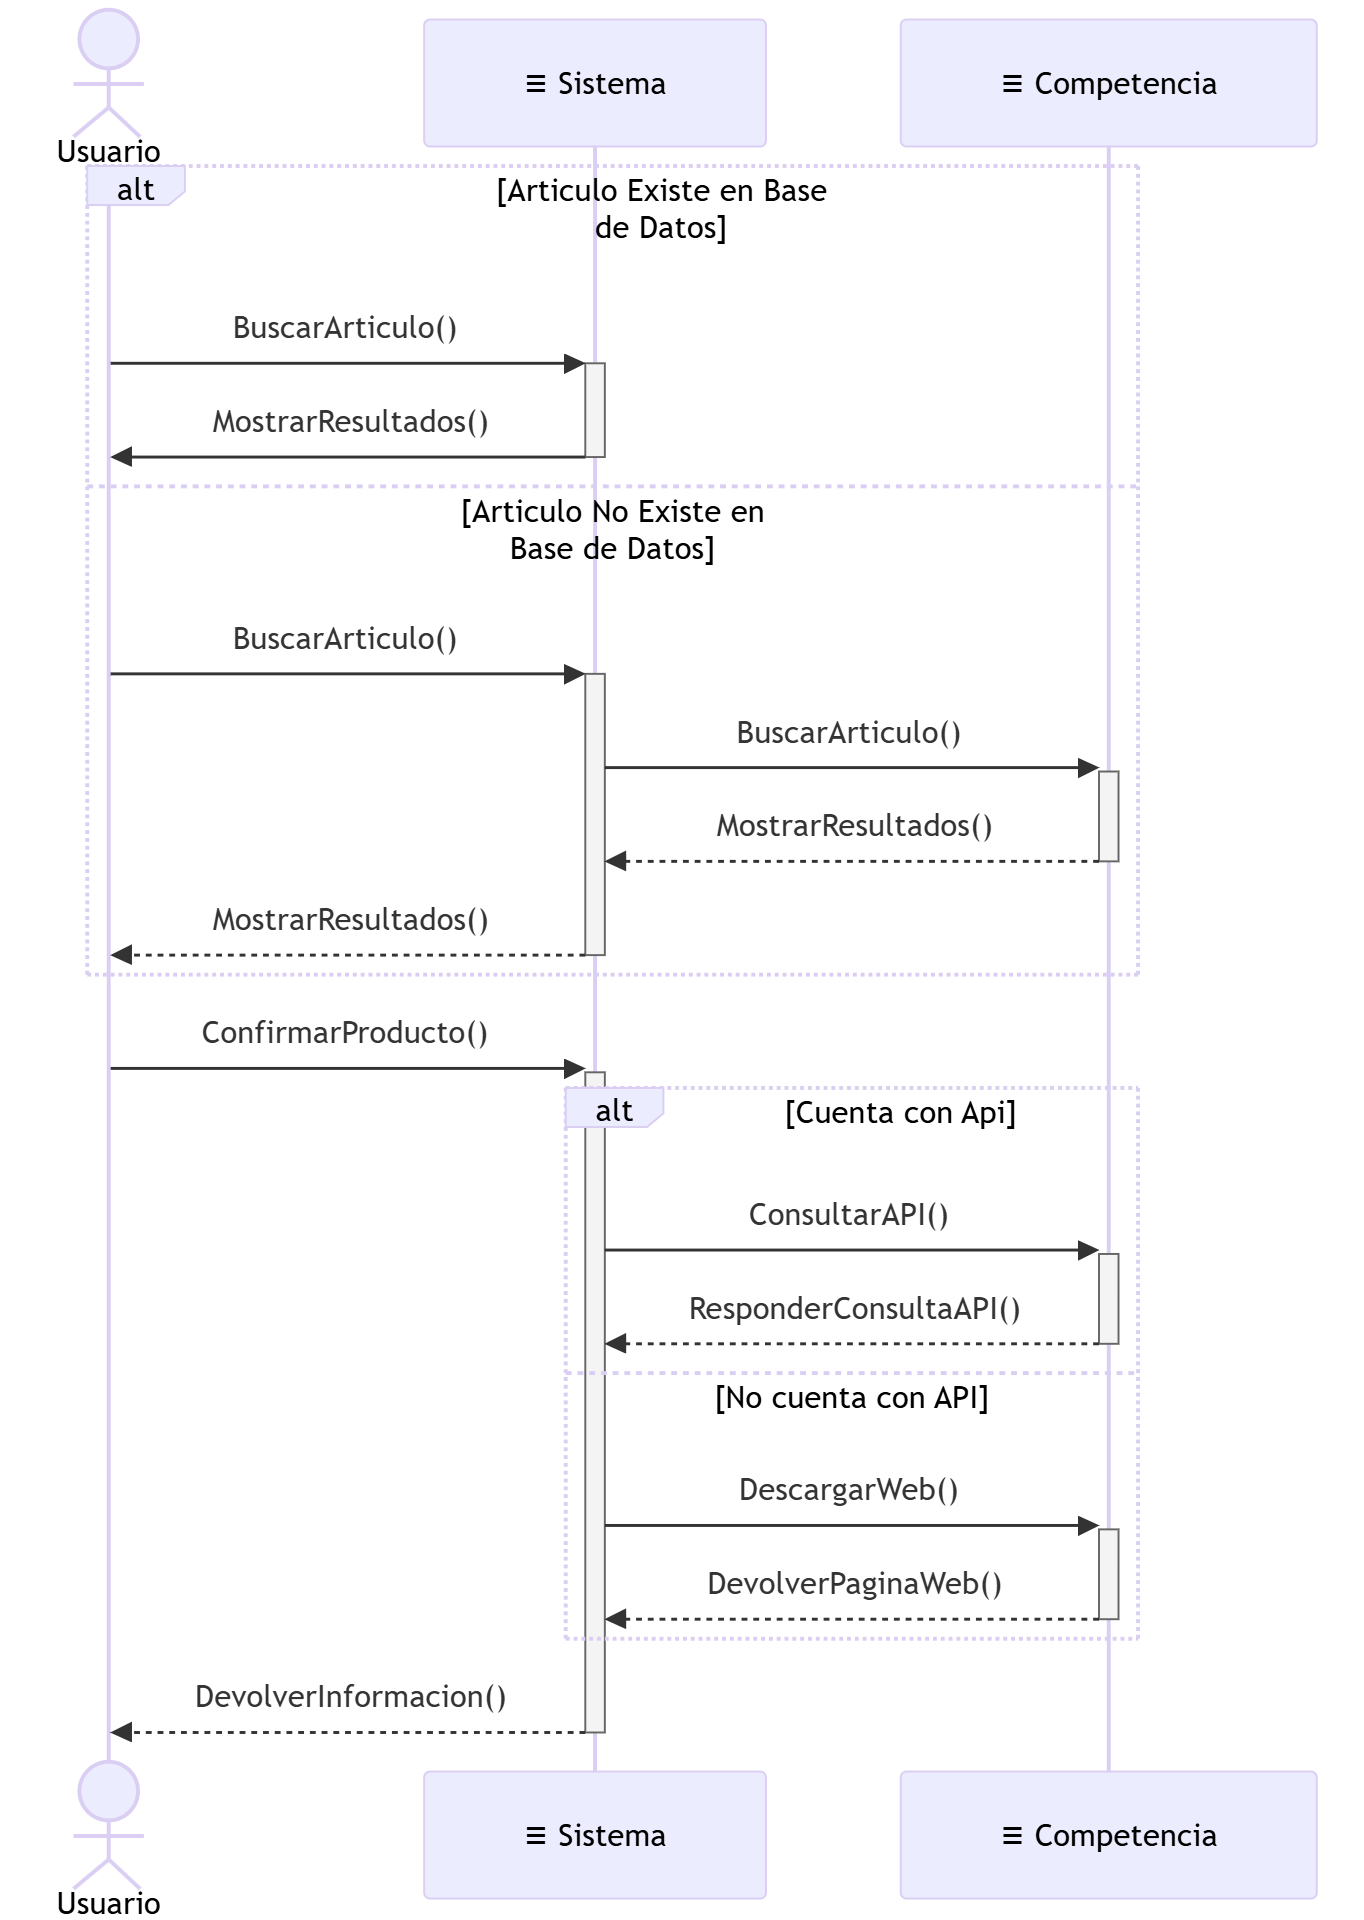
\includegraphics[width=.9\textwidth]{img/04-diagrama-caso-2.png}
	\vspace{15pt}
\end{figure}

\pagebreak

\subsection{Seguir el stock disponible, previendo necesidades de corto y mediano plazo.}

\textbf{Resumen:}
Dado número de parte,
nombre o descripción,
en forma íntegra o parcial,
el encargado de compras debe contar con un número de stock disponible de un producto y,
de ser necesario,
actualizar el stock.

\textbf{Precondición:} 
el encargado de compras ingresa -de manera parcial o completa- el nombre, descripción o número de parte de un producto

\textbf{Escenario principal:}
\begin{enumerate}
	\item El encargado de compras ingresa a la sección de stock del sistema.
	\item El sistema solicita el ingreso de número de parte, descripción o nombre del producto.
	\item El encargado de compras ingresa cualquiera de los datos, de forma completa o parcial.
	\item El sistema muestra coincidencias al encargado de compras, de manera tal que elija el artículo buscado.
	\item El encargado de compras confirma el producto buscado.
	\item El sistema devuelve la información relativa al producto almacenada en base de datos,
	incluyendo nombre, descripción, último precio de compra, último precio de venta y stock.
	A continuación, solicita al usuario confirmar si desea hacer una modificación al stock.
	\item El usuario confirma que desea modificar el stock e incorpora la cantidad disponible del producto en depósito.
\end{enumerate}

\textbf{Poscondición:}
El encargado de compras dispone, en tiempo real,
de la cantidad de stock disponible
y del resto de la información sobre el producto,
así como la posibilidad de modificar la información relativa al stock.

\textbf{Flujo alternativo:}

\textbf{A1} El nombre, descripción o número de parte no coincide con ningún producto en base de datos.

La secuencia comienza en el punto 3.

\begin{enumerate}
	\item[4.] El sistema informa que no existen coincidencias con productos en base de datos,
	y solicita cargar número de parte íntegramente para buscar por nomenclador único.
	\item[5.] El encargado de compras carga el número de parte, esta vez de forma íntegra,
	para garantizar que encuentra el producto deseado.
\end{enumerate}

El escenario vuelve a punto 4.

\textbf{A2} Nuevamente, aún con nomenclador único, el sistema no encuentra el producto en base de datos.

La secuencia comienza en el punto 5 del flujo alternativo \textbf{A1}.

\begin{enumerate}
	\item [7.] El sistema informa que dicho número de parte no coincide con ningún producto en base de datos, 
	solicita corroborar dicho número y asegurarse de que el producto existe en base de datos.
\end{enumerate}

El escenario vuelve al punto 2.

\begin{figure}[H]
	\centering
	\vspace{15pt}
	\caption{Caso de Uso 3, incluyendo Flujos Alternativos}
	\vspace{15pt}
	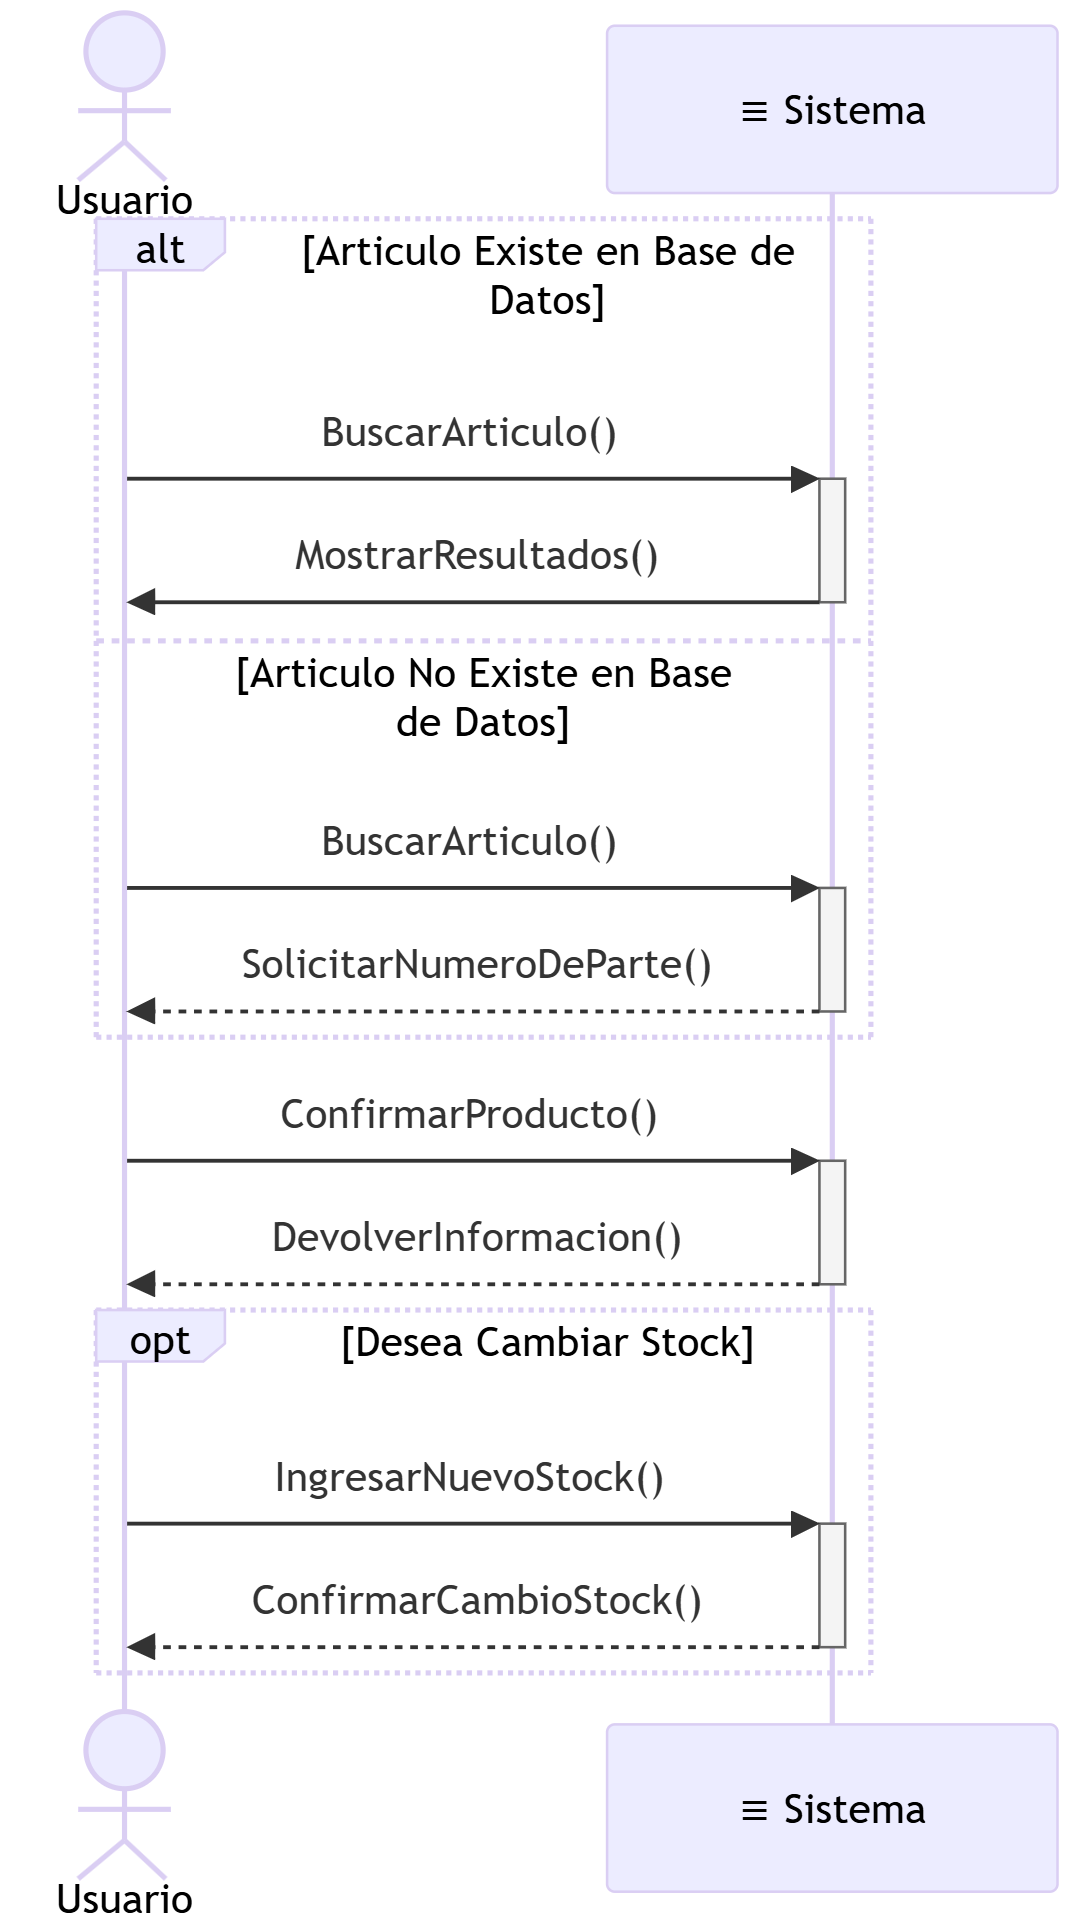
\includegraphics[width=.7\textwidth]{img/04-diagrama-caso-3.png}
	\vspace{15pt}
\end{figure}

\pagebreak

\subsection{Conocer los precios de recompra para un producto}
 
\textbf{Resumen:}
El encargado de ventas puede necesitar la información del costo de recompra de un producto,
para reaccionar a un cambio en el precio de mercado.
En ocasiones, un precio de mercado de un producto puede caer,
y el encargado de ventas debe ser capaz de reaccionar a ello.
Este precio se tomará del fijado por el encargado de compras.

\textbf{Precondición:} 
El encargado de ventas ingresa, completo o de manera parcial, el nombre, descripción o número de parte de un producto.

\textbf{Escenario principal:}
\begin{enumerate}
	\item El encargado de ventas ingresa a la sección de \textbf{precios de compra} del sistema.
	\item El sistema solicita el ingreso de número de parte, descripción o nombre del producto.
	\item El encargado de ventas ingresa cualquiera de los datos, de forma completa o parcial.
	\item El sistema muestra las coincidencias, de manera tal que el usuario elija el artículo buscado.
	\item El usuario confirma el producto buscado.
	\item El sistema devuelve la información relativa al producto almacenada en base de datos,
	incluyendo nombre, descripción, último precio de venta, stock y último precio de compra.
\end{enumerate}

\textbf{Poscondición:}
El encargado de ventas dispone, en tiempo real,
de toda la información almacenada referida al producto,
en particular,
del último precio de compra,
informado por el encargado de compras.

\textbf{Flujo alternativo:}

\textbf{A1} El nombre, descripción o número de parte no coincide con ningún producto en base de datos.

La secuencia comienza en el punto 3.

\begin{enumerate}
	\item[4.] El sistema informa que no existen coincidencias con productos en base de datos,
	y solicita cargar número de parte íntegramente para buscar por nomenclador único.
	\item[5.] El usuario carga el número de parte, esta vez de forma íntegra,
	para garantizar que encuentra el producto deseado.
\end{enumerate}

El escenario vuelve a punto 4.

\textbf{A2} Nuevamente, aún con número de parte, el sistema no encuentra el producto en base de datos.

La secuencia comienza en el punto 5 del flujo alternativo \textbf{A1}.

\begin{enumerate}
	\item [7.] El sistema informa que dicho número de parte no coincide con ningún producto en base de datos, 
	solicita corroborar dicho número y asegurarse de que el producto existe en base de datos.
	En caso contrario, debe informarse al encargado de compras, quien es el único usuario autorizado a incorporar productos a base de datos.
\end{enumerate}

El escenario vuelve al punto 2.

\begin{figure}[H]
	\centering
	\vspace{15pt}
	\caption{Caso de Uso 4, incluyendo Flujos Alternativos}
	\vspace{15pt}
	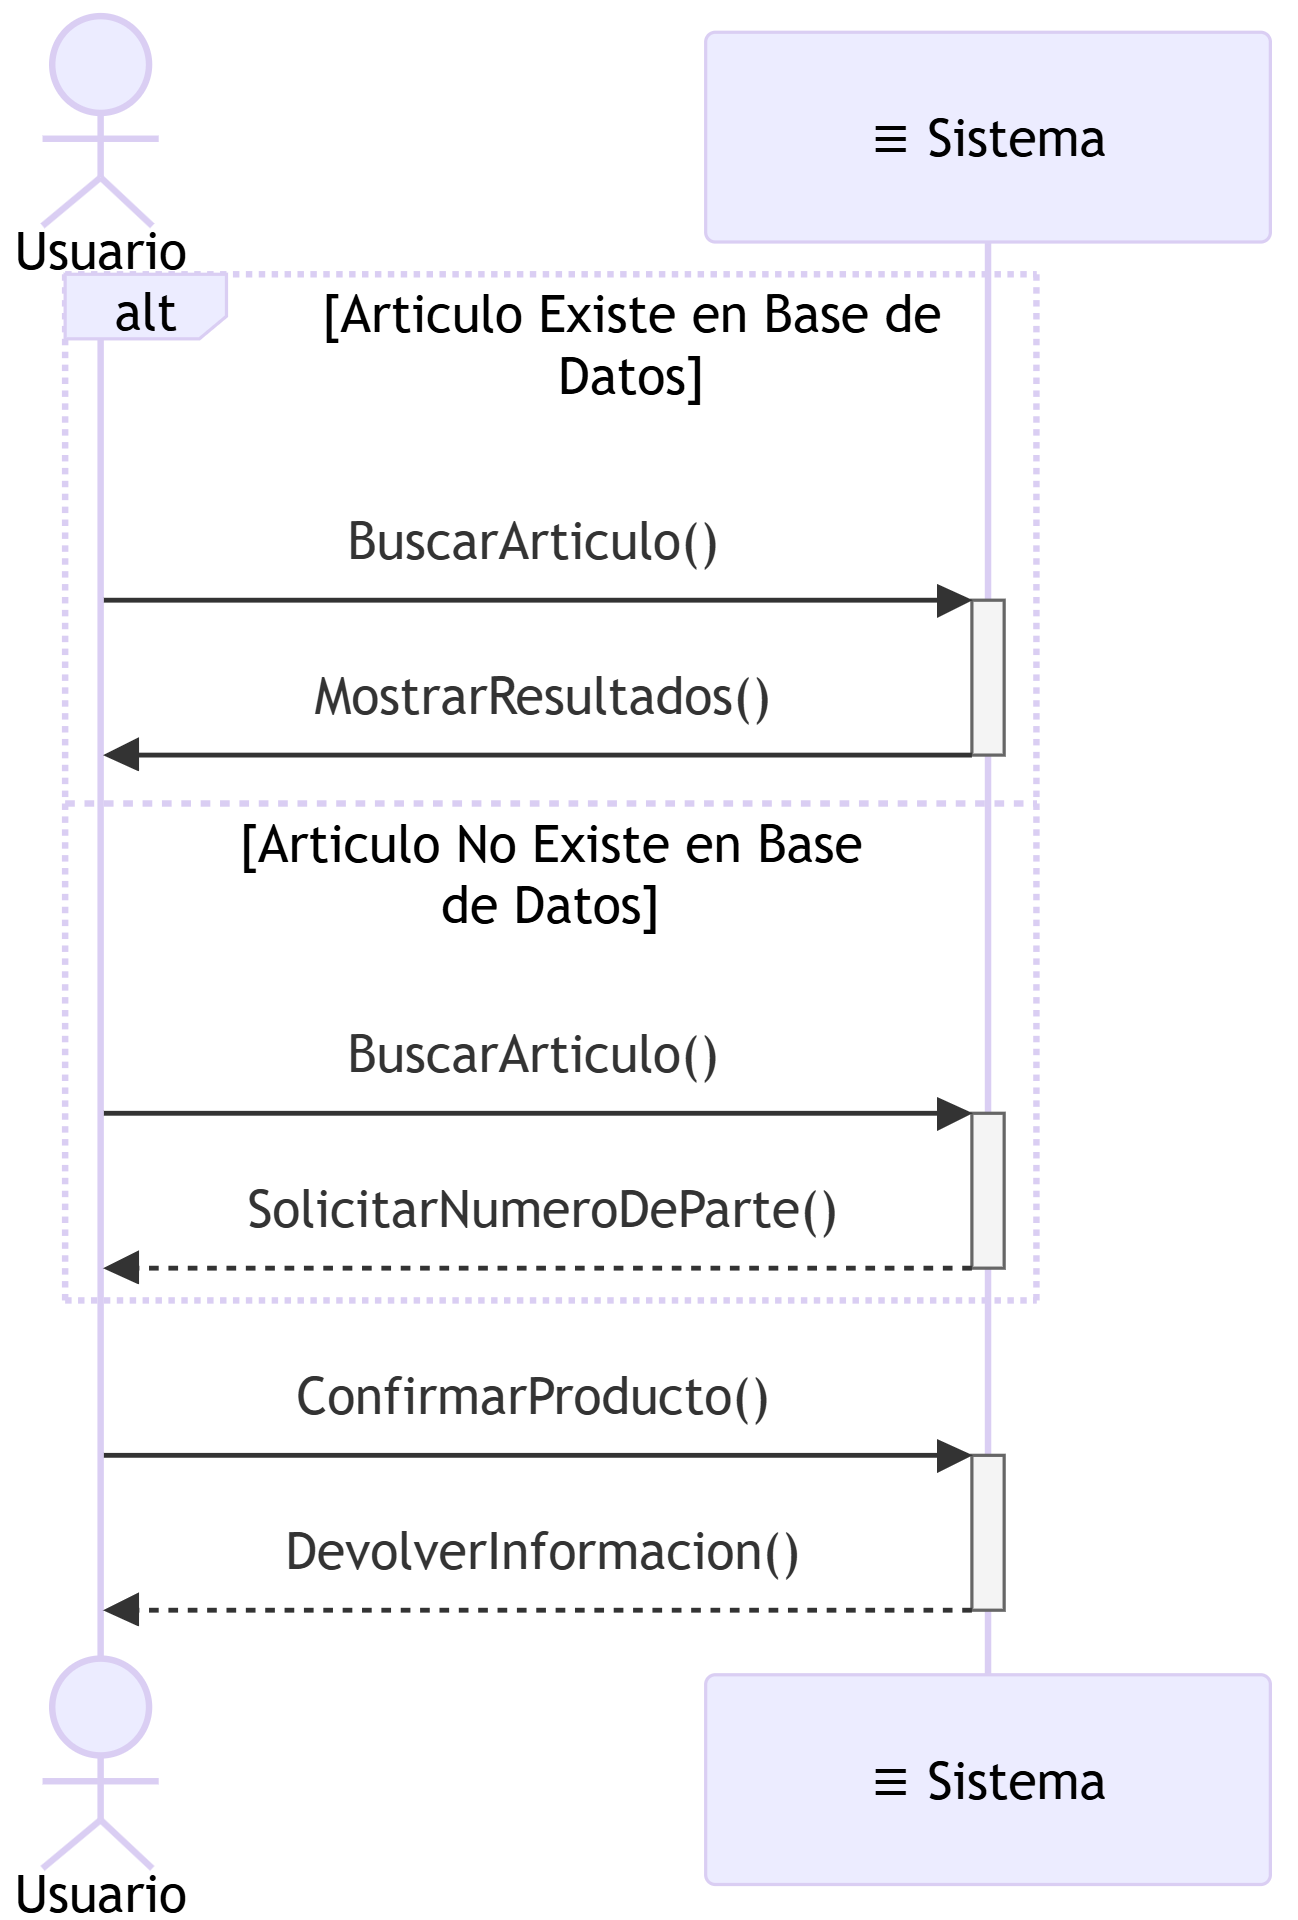
\includegraphics[width=.7\textwidth]{img/04-diagrama-caso-4.png}
	\vspace{15pt}
\end{figure}

\pagebreak

\subsection{Conocer los precios de la competencia}

\textbf{Resumen:}
Para determinar un precio competitivo,
que cuide a los clientes al tiempo que asegura rentabilidad a la empresa,
el encargado de ventas debe de disponer del precio de mercado.
Para ello, 
dado un número de parte,
nombre o descripción,
el encargado de ventas contará con un listado de precios,
obtenido de portales de venta de la competencia, 
como son Mercado Libre, Amazon y otros.
Con esta información, 
el encargado de ventas definirá los precios de lista de los productos,
que será el precio al consumidor final.

\textbf{Precondición:} 
el usuario ingresa parte del nombre/descripción/número de parte en el sistema,
en la sección correspondiente a \textbf{precios de venta},
para iniciar una búsqueda

\textbf{Escenario principal:}
\begin{enumerate}
	\item El usuario ingresa a la opción búsqueda de precios de venta.
	\item El sistema solicita ingreso de número de parte, descripción o nombre, del producto.
	\item El usuario ingresa cualquiera de los datos, de forma completa o parcial.
	\item El sistema muestra coincidencias al usuario, quien deberá elegir el artículo buscado.
	\item El usuario confirma el producto buscado.
	\item El sistema descarga la información necesaria, 
	recurriendo en los casos en que sea posible a las interfaces de programación de los proveedores (API),
	al \textit{Web Scrapping} donde no sea posible. Una vez recopilada la información, 
	se presenta al usuario por nombre de portal de venta y precio.
	\item El encargado toma las decisiones correspondientes.
\end{enumerate}

\textbf{Poscondición:}
El encargado de ventas dispone de información suficiente, en tiempo real, para fijar un precio que equilibre rendimiento y competitividad.

\textbf{Flujo alternativo:}

\textbf{A1} El nombre, descripción o número de parte no coincide con un producto cargado en base de datos.

La secuencia comienza en el punto 3.

\begin{enumerate}
	\item[4.] El sistema informa que no existen coincidencias con productos en base de datos,
	y solicita cargar número de parte íntegramente para buscar por nomenclador único.
	\item[5.] El usuario carga número de parte íntegramente.
	\item[6.] El sistema muestra coincidencias.
\end{enumerate}

El escenario vuelve a punto 5.

\textbf{A2} El nombre, descripción o número de parte no coincide con ningún producto, ni en base de datos ni en proveedor

La secuencia comienza en el punto 6 del flujo alternativo \textbf{A1}.

\begin{enumerate}
	\item [7.] El sistema informa que dicho número de parte no coincide con ningún producto en base de datos,
	solicita corroborar dicho número y asegurarse de que el producto existe en base de datos.
	En caso contrario, debe informarse al encargado de compras, quien es el único usuario autorizado a incorporar productos a base de datos.
\end{enumerate}

El escenario vuelve al punto 2.

\begin{figure}[H]
	\centering
	\vspace{15pt}
	\caption{Caso de Uso 5, incluyendo Flujos Alternativos}
	\vspace{15pt}
	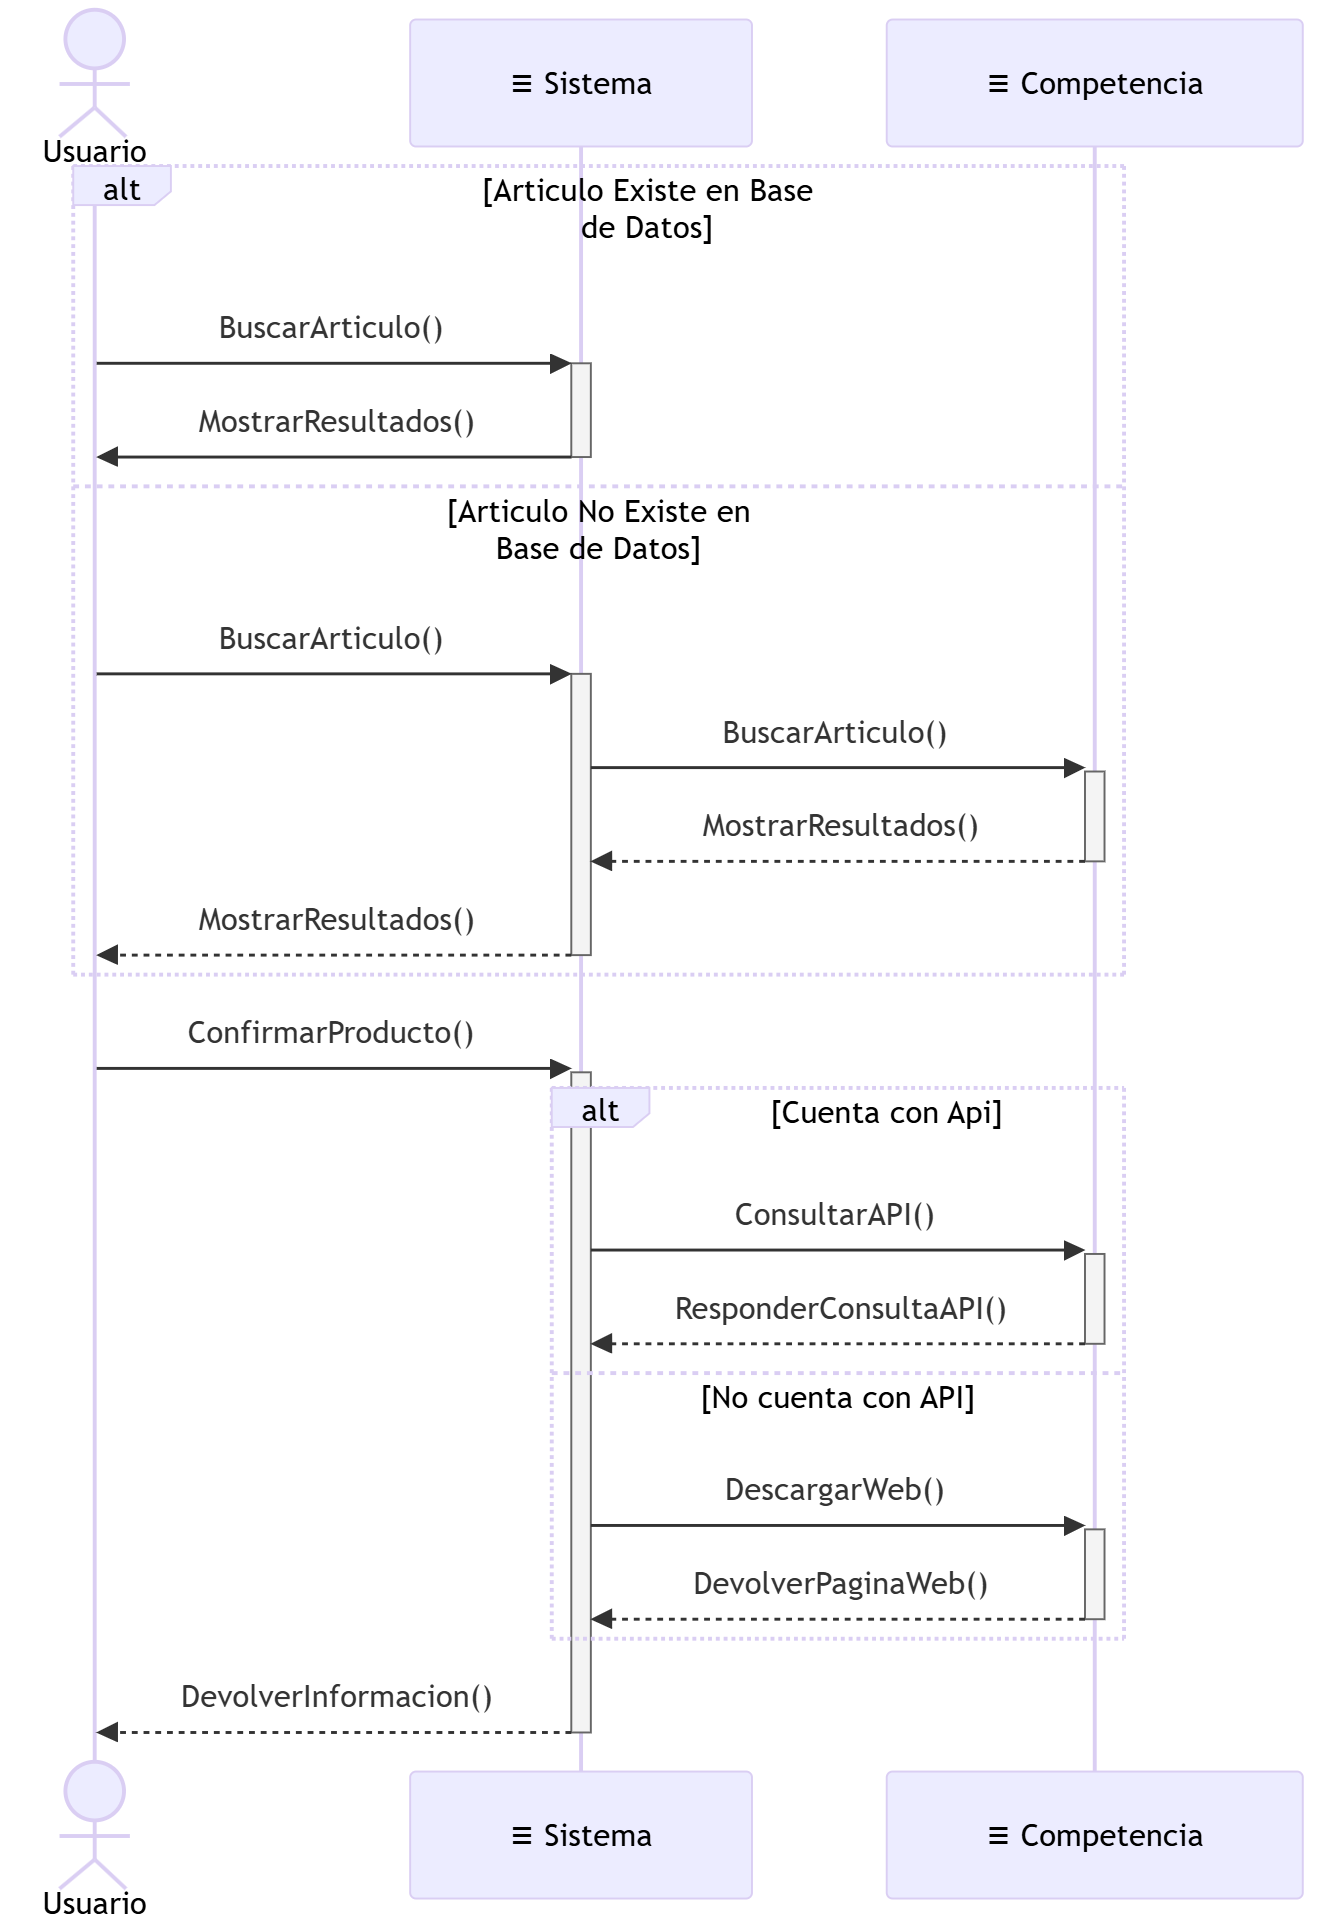
\includegraphics[width=.8\textwidth]{img/04-diagrama-caso-5.png}
	\vspace{15pt}
\end{figure}

\pagebreak

\subsection{Fijar precio para un producto}

\textbf{Resumen:}
Conociendo precio de recompra y precio de mercado,
el encargado de ventas fijará un precio de lista a consumidor final de un producto,
procurando un equilibrio entre competitividad y rentabilidad.
El precio de lista fijado para un producto será luego leído por el personal de ventas,
para la atención al público y la emisión de factura electrónica.

\textbf{Precondición:} 
el encargado de ventas ingresa -de manera parcial o completa- el nombre, descripción o número de parte de un producto

\textbf{Escenario principal:}
\begin{enumerate}
	\item El usuario ingresa a la sección de precios de venta (también denominado precio de lista) del sistema.
	\item El sistema solicita el ingreso de número de parte, descripción o nombre del producto.
	\item El usuario ingresa cualquiera de los datos, de forma completa o parcial.
	\item El sistema muestra coincidencias al usuario, de manera tal que elija el artículo buscado.
	\item El usuario confirma el producto buscado.
	\item El sistema devuelve la información relativa al producto almacenada en base de datos,
	incluyendo nombre, descripción, último precio de compra, último precio de venta y stock.
	A continuación, solicita al usuario confirmar si desea hacer una modificación al precio de venta.
	\item El usuario confirma que desea modificar el precio de venta e ingresa el mismo a la interfaz del sistema.
	\item El sistema almacena el nuevo precio de venta, que será utilizado en adelante por el personal de ventas.
\end{enumerate}

\textbf{Poscondición:}
El encargado de ventas dispone, en tiempo real,
de la posibilidad de fijar el precio de un producto,
así como la posibilidad de observar toda la información relativa al mismo que es almacenada en base de datos.

\textbf{Flujo alternativo:}

\textbf{A1} El nombre, descripción o número de parte no coincide con ningún producto en base de datos.

La secuencia comienza en el punto 3.

\begin{enumerate}
	\item[4.] El sistema informa que no existen coincidencias con productos en base de datos,
	y solicita cargar número de parte íntegramente para buscar por nomenclador único.
	\item[5.] El usuario carga el número de parte, esta vez de forma íntegra,
	para garantizar que encuentra el producto deseado.
\end{enumerate}

El escenario vuelve a punto 4.

\textbf{A2} Nuevamente, aún con nomenclador único, el sistema no encuentra el producto en base de datos.

La secuencia comienza en el punto 5 del flujo alternativo \textbf{A1}.

\begin{enumerate}
	\item [6.] El sistema informa que dicho número de parte no coincide con ningún producto en base de datos, 
	solicita corroborar dicho número y asegurarse de que el producto existe en base de datos.
	En caso contrario, debe informarse al encargado de compras, quien es el único usuario autorizado a incorporar productos a base de datos.
\end{enumerate}

El escenario vuelve al punto 2.

\begin{figure}[H]
	\centering
	\vspace{15pt}
	\caption{Caso de Uso 6, incluyendo Flujos Alternativos}
	\vspace{15pt}
	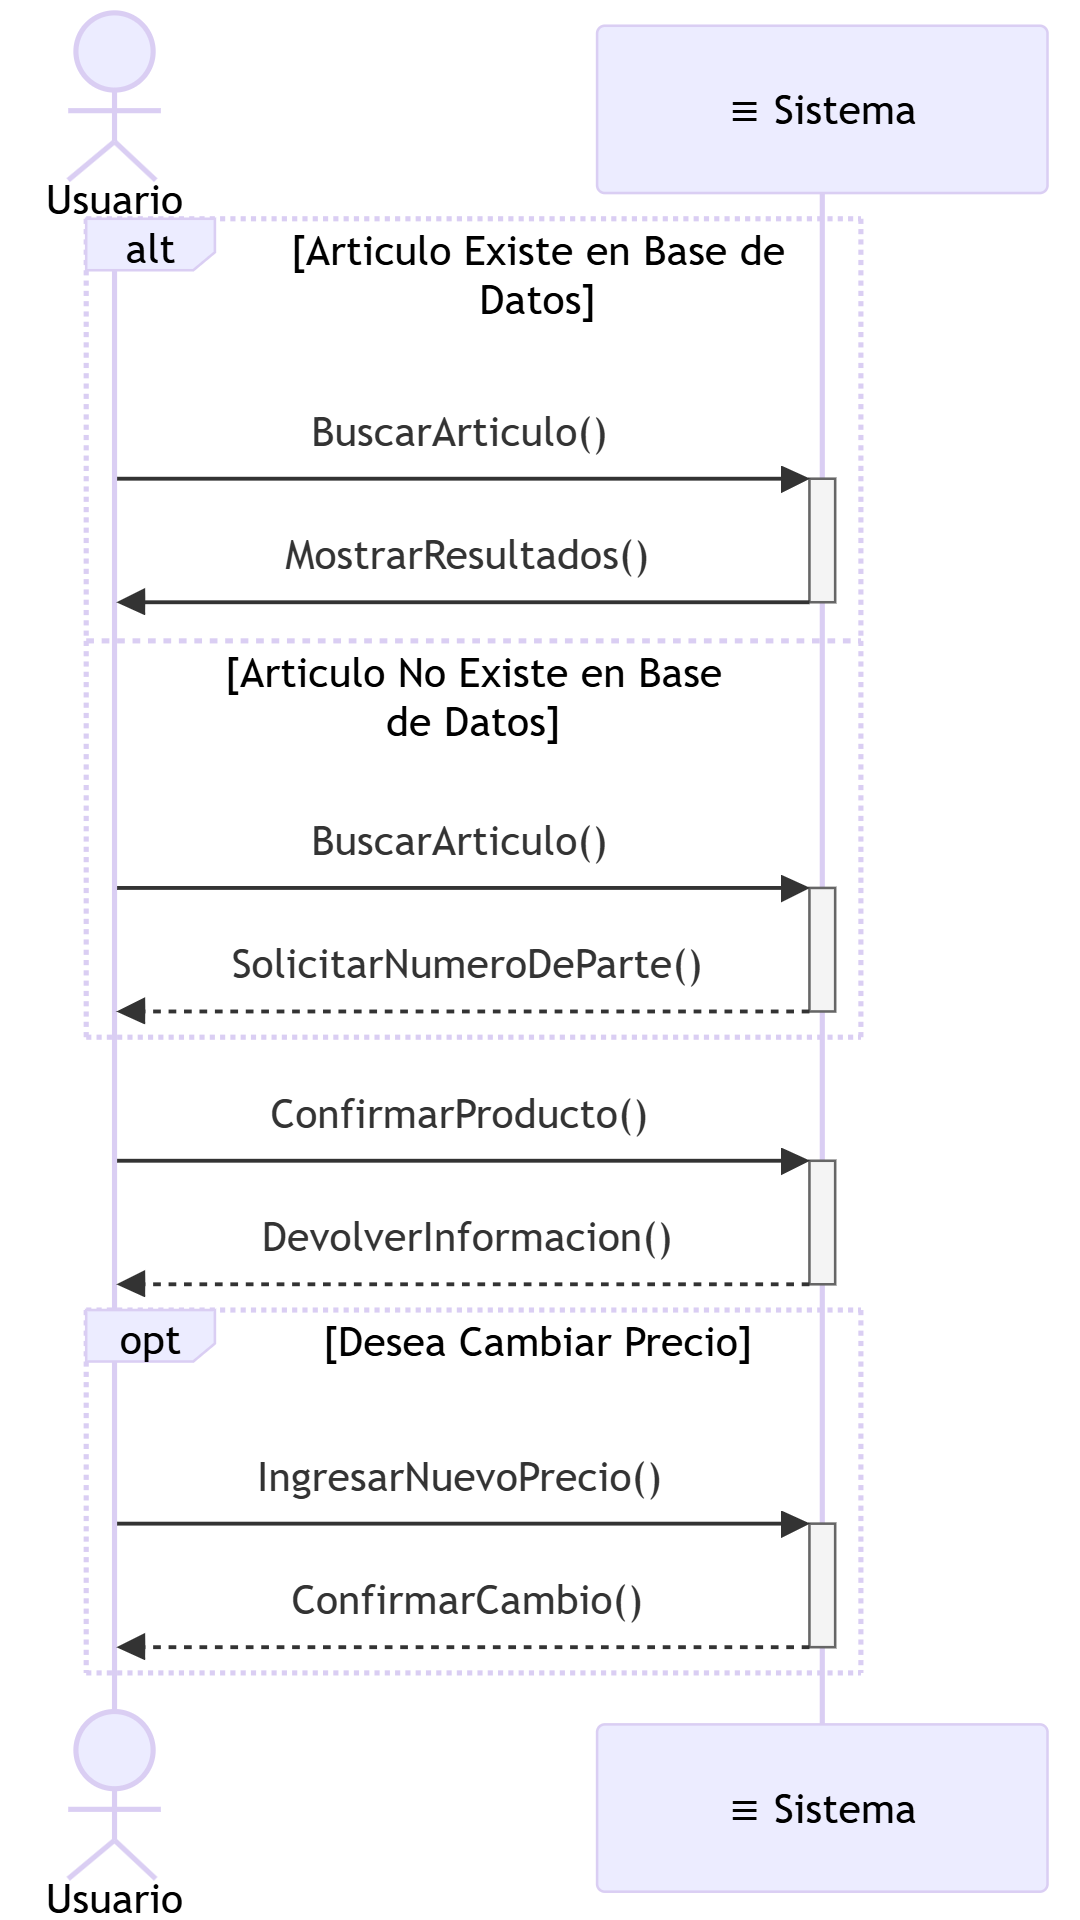
\includegraphics[width=.6\textwidth]{img/04-diagrama-caso-6.png}
	\vspace{15pt}
\end{figure}

\pagebreak

\subsection{Consultar precio de un producto}

\textbf{Resumen:}
El personal de venta atiende al comprador minorista y debe consultar el último precio de venta,
fijado ya por el encargado de ventas.
Estos precios pueden variar con relativa velocidad,
tanto al alza por una escasez relativa,
como a la baja para reaccionar a la creciente competencia,
y el personal de ventas debe estar sincronizado con dichos cambios.

\textbf{Precondición:} 
Personal de ventas, en el proceso de atención y asesoramiento correspondiente,
requiere consultar el precio de lista (también denominado precio de venta)
de un producto.

\textbf{Escenario principal:}
\begin{enumerate}
	\item Personal de ventas ingresa a la sección de emisión de factura electrónica (aunque aún no se vaya a emitir, la interfaz debe ser la misma).
	\item El sistema solicita ingresar identificación de cliente, mediante CUIT o código interno alfanumérico.
	\item Personal de ventas ingresa identificación de cliente o nomenclador por categoría, como CF para consumidor final.
	\item El sistema, de acuerdo a la identificación del cliente, determina si la boleta será tipo A o tipo B.
	\item El sistema, luego de determinar el tipo de factura, solicita ingresar el primer producto.
	\item Personal de ventas ingresa el producto, por número de parte, nombre, código de barras o descripción, de manera completa o parcial.
	\item El sistema muestra las coincidencias en base de datos, esperando confirmación.
	\item Personal de ventas confirma la coincidencia e ingresa cantidad.
	\item El sistema muestra el precio unitario y total, de acuerdo a la cantidad ingresada.
	Además, si el usuario desea incorporar otro producto, vuelve al punto 5.
\end{enumerate}

\textbf{Poscondición:}
Personal de ventas tiene el precio unitario y total correspondiente al producto solicitado por el cliente.

\textbf{Flujo alternativo:}

\textbf{A1} El personal de ventas ingresa el CUIT del cliente, pero este no está cargado en base de datos

Secuencia comienza en punto 3

\begin{enumerate}
	\item[4.] El sistema hace una petición al sistema de ARCA de los datos del contribuyente, 
	empleando el CUIT para identificarlo.
	\item[5.] ARCA devuelve los datos del contribuyente.
	\item[6.] El sistema los incorpora a la base de datos.
\end{enumerate}

Vuelve al escenario principal en punto 4

\textbf{A2} Personal de ventas ingresa un producto, pero este no existe en base de datos

Secuencia comienza en 6.

\begin{enumerate}
	\item[7.] El sistema no encuentra coincidencias, por lo que pide reingreso al personal de ventas.
	\item[8.] Personal de ventas prueba con descripción, código de barras o ingreso manual de nombenclador.
\end{enumerate}

Vuelve a flujo normal en punto 8.

\textbf{A2} El cliente desea un comprobante tipo presupuesto impreso

Secuencia comienza en 9.

\begin{enumerate}
	\item[10.] El usuario solicita imprimir comprobante sin autorizar, formato presupuesto.
	\item[11.] El sistema transmite la información correspondiente al módulo de impresión predeterminado del sistema operativo,
	que manejará el proceso de impresión.
\end{enumerate}

\pagebreak

\begin{figure}[H]
	\centering
	\vspace{15pt}
	\caption{Caso de Uso 7, incluyendo Flujos Alternativos}
	\vspace{15pt}
	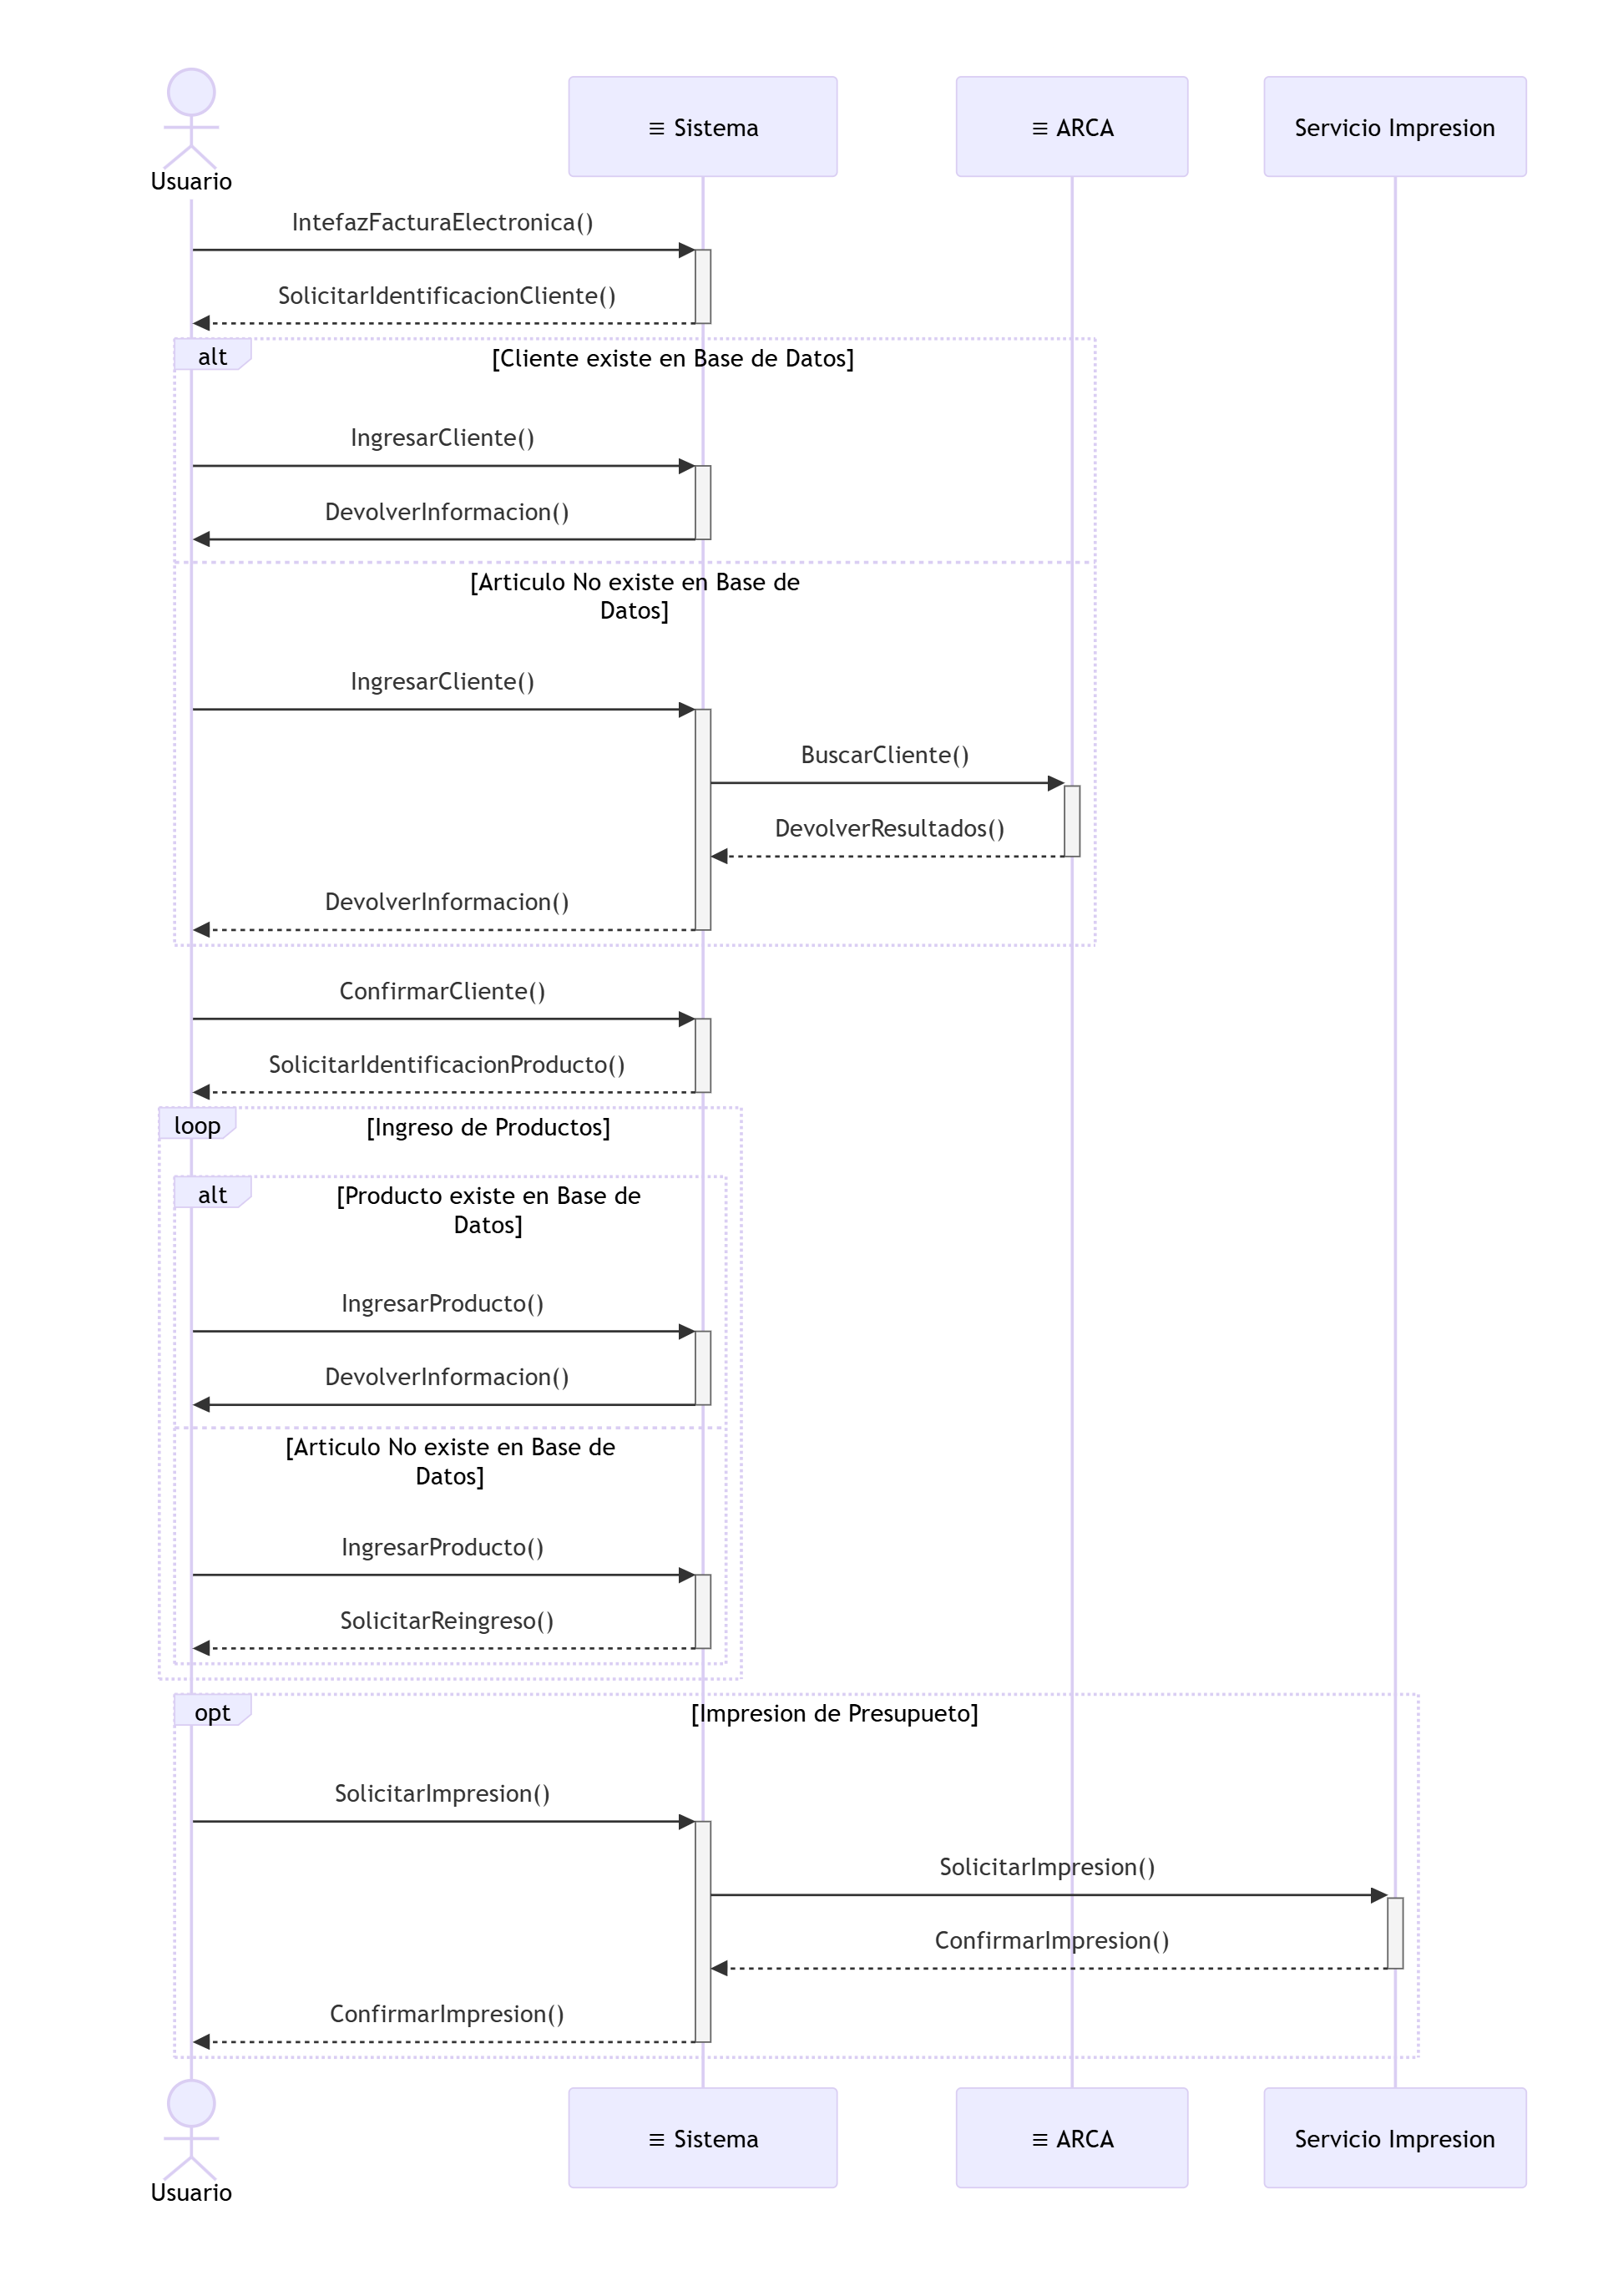
\includegraphics[width=.95\textwidth]{img/04-diagrama-caso-7.png}
	\vspace{15pt}
\end{figure}

\pagebreak

\subsection{Confirmar disponibilidad de stock de producto al consumidor final que lo requiera.}

\textbf{Resumen:}
En la atención al cliente minorista,
el personal de venta debe disponer de información relativa a los stocks,
para confirmar existencia de producto en depósito.

Este caso de uso mantiene una relación tipo \texttt{include} con el anterior.

\pagebreak

\subsection{Emitir factura electrónica}

\textbf{Resumen:}
Personal de venta, 
luego de la brindar atención y asesoramiento al comprador minorista,
requiere de la información del sistema
-descripción del producto, cantidad, disponibilidad y precio-
para emitir una factura electrónica.
Esto puede hacerse sincronizando al sistema con la API de la ex AFIP,
ahora ARCA.

\textbf{Actores:} Personal de ventas (primario), Sistema de ARCA (secundario).

\textbf{Precondición:} 
Personal de ventas ha concluido con la atención y asesoramiento correspondiente,
el cliente minorista decide proceder con la compra,
por lo cual el personal de ventas solicita iniciar el procedimiento para emitir factura electrónica.

\textbf{Escenario principal:}
\begin{enumerate}
	\item Personal de ventas ingresa a la sección de emisión de factura electrónica
	\item El sistema solicita ingresar identificación de cliente, mediante CUIT o código interno alfanumérico.
	\item Personal de ventas ingresa identificación de cliente o nomenclador por categoría, como CF para consumidor final.
	\item El sistema, de acuerdo a la identificación del cliente, determina si la boleta será tipo A o tipo B.
	\item El sistema, luego de determinar el tipo de factura, solicita ingresar el primer producto.
	\item Personal de ventas ingresa el producto, por número de parte, código de barras o descripción.
	\item El sistema muestra las coincidencias en base de datos, esperando confirmación.
	\item Personal de ventas confirma la coincidencia e ingresa cantidad.
	\item El sistema aguarda la carga de nuevo item, en dicho caso vuelve a punto 6.
	\item Personal de ventas indica que finaliza la carga de productos, solicitando autorización de comprobante.
	\item El sistema envía petición a servicio de ARCA, incluyendo: CUIT de cliente, cantidad de productos, Iva y precio final.
	\item Servidor de ARCA confirma autorización de boleta, devolviendo número de comprobante electrónico.
	\item El sistema solicita al personal de ventas confirme para imprimir el comprobante o exportarlo a PDF.
	\item Personal de ventas confirma y obtiene el comprobante en el formato deseado.
\end{enumerate}

\textbf{Poscondición:}
Personal de ventas tiene el comprobante correspondiente a la compra del cliente y puede finalizar el proceso de compra entregando comprobante y producto.

\textbf{Flujo alternativo:}

\textbf{A1} El personal de ventas ingresa el CUIT del cliente, pero este no está cargado en base de datos

Secuencia comienza en punto 3

\begin{enumerate}
	\item[4.] El sistema hace una petición al sistema de ARCA de los datos del contribuyente, 
	empleando el CUIT para identificarlo.
	\item[5.] ARCA devuelve los datos del contribuyente.
	\item[6.] El sistema los incorpora a la base de datos.
\end{enumerate}

Vuelve al escenario principal en punto 4

\textbf{A2} Personal de ventas ingresa un producto, pero este no existe en base de datos

Secuencia comienza en 6.

\begin{enumerate}
	\item[7.] El sistema no encuentra coincidencias, por lo que pide reingreso al personal de ventas.
	\item[8.] Personal de ventas prueba con descripción, código de barras o ingreso manual de nombenclador.
\end{enumerate}

Vuelve a flujo normal en punto 8.

\pagebreak

\begin{figure}[H]
	\centering
	\vspace{15pt}
	\caption{Caso de Uso 8, incluyendo Flujos Alternativos}
	\vspace{15pt}
	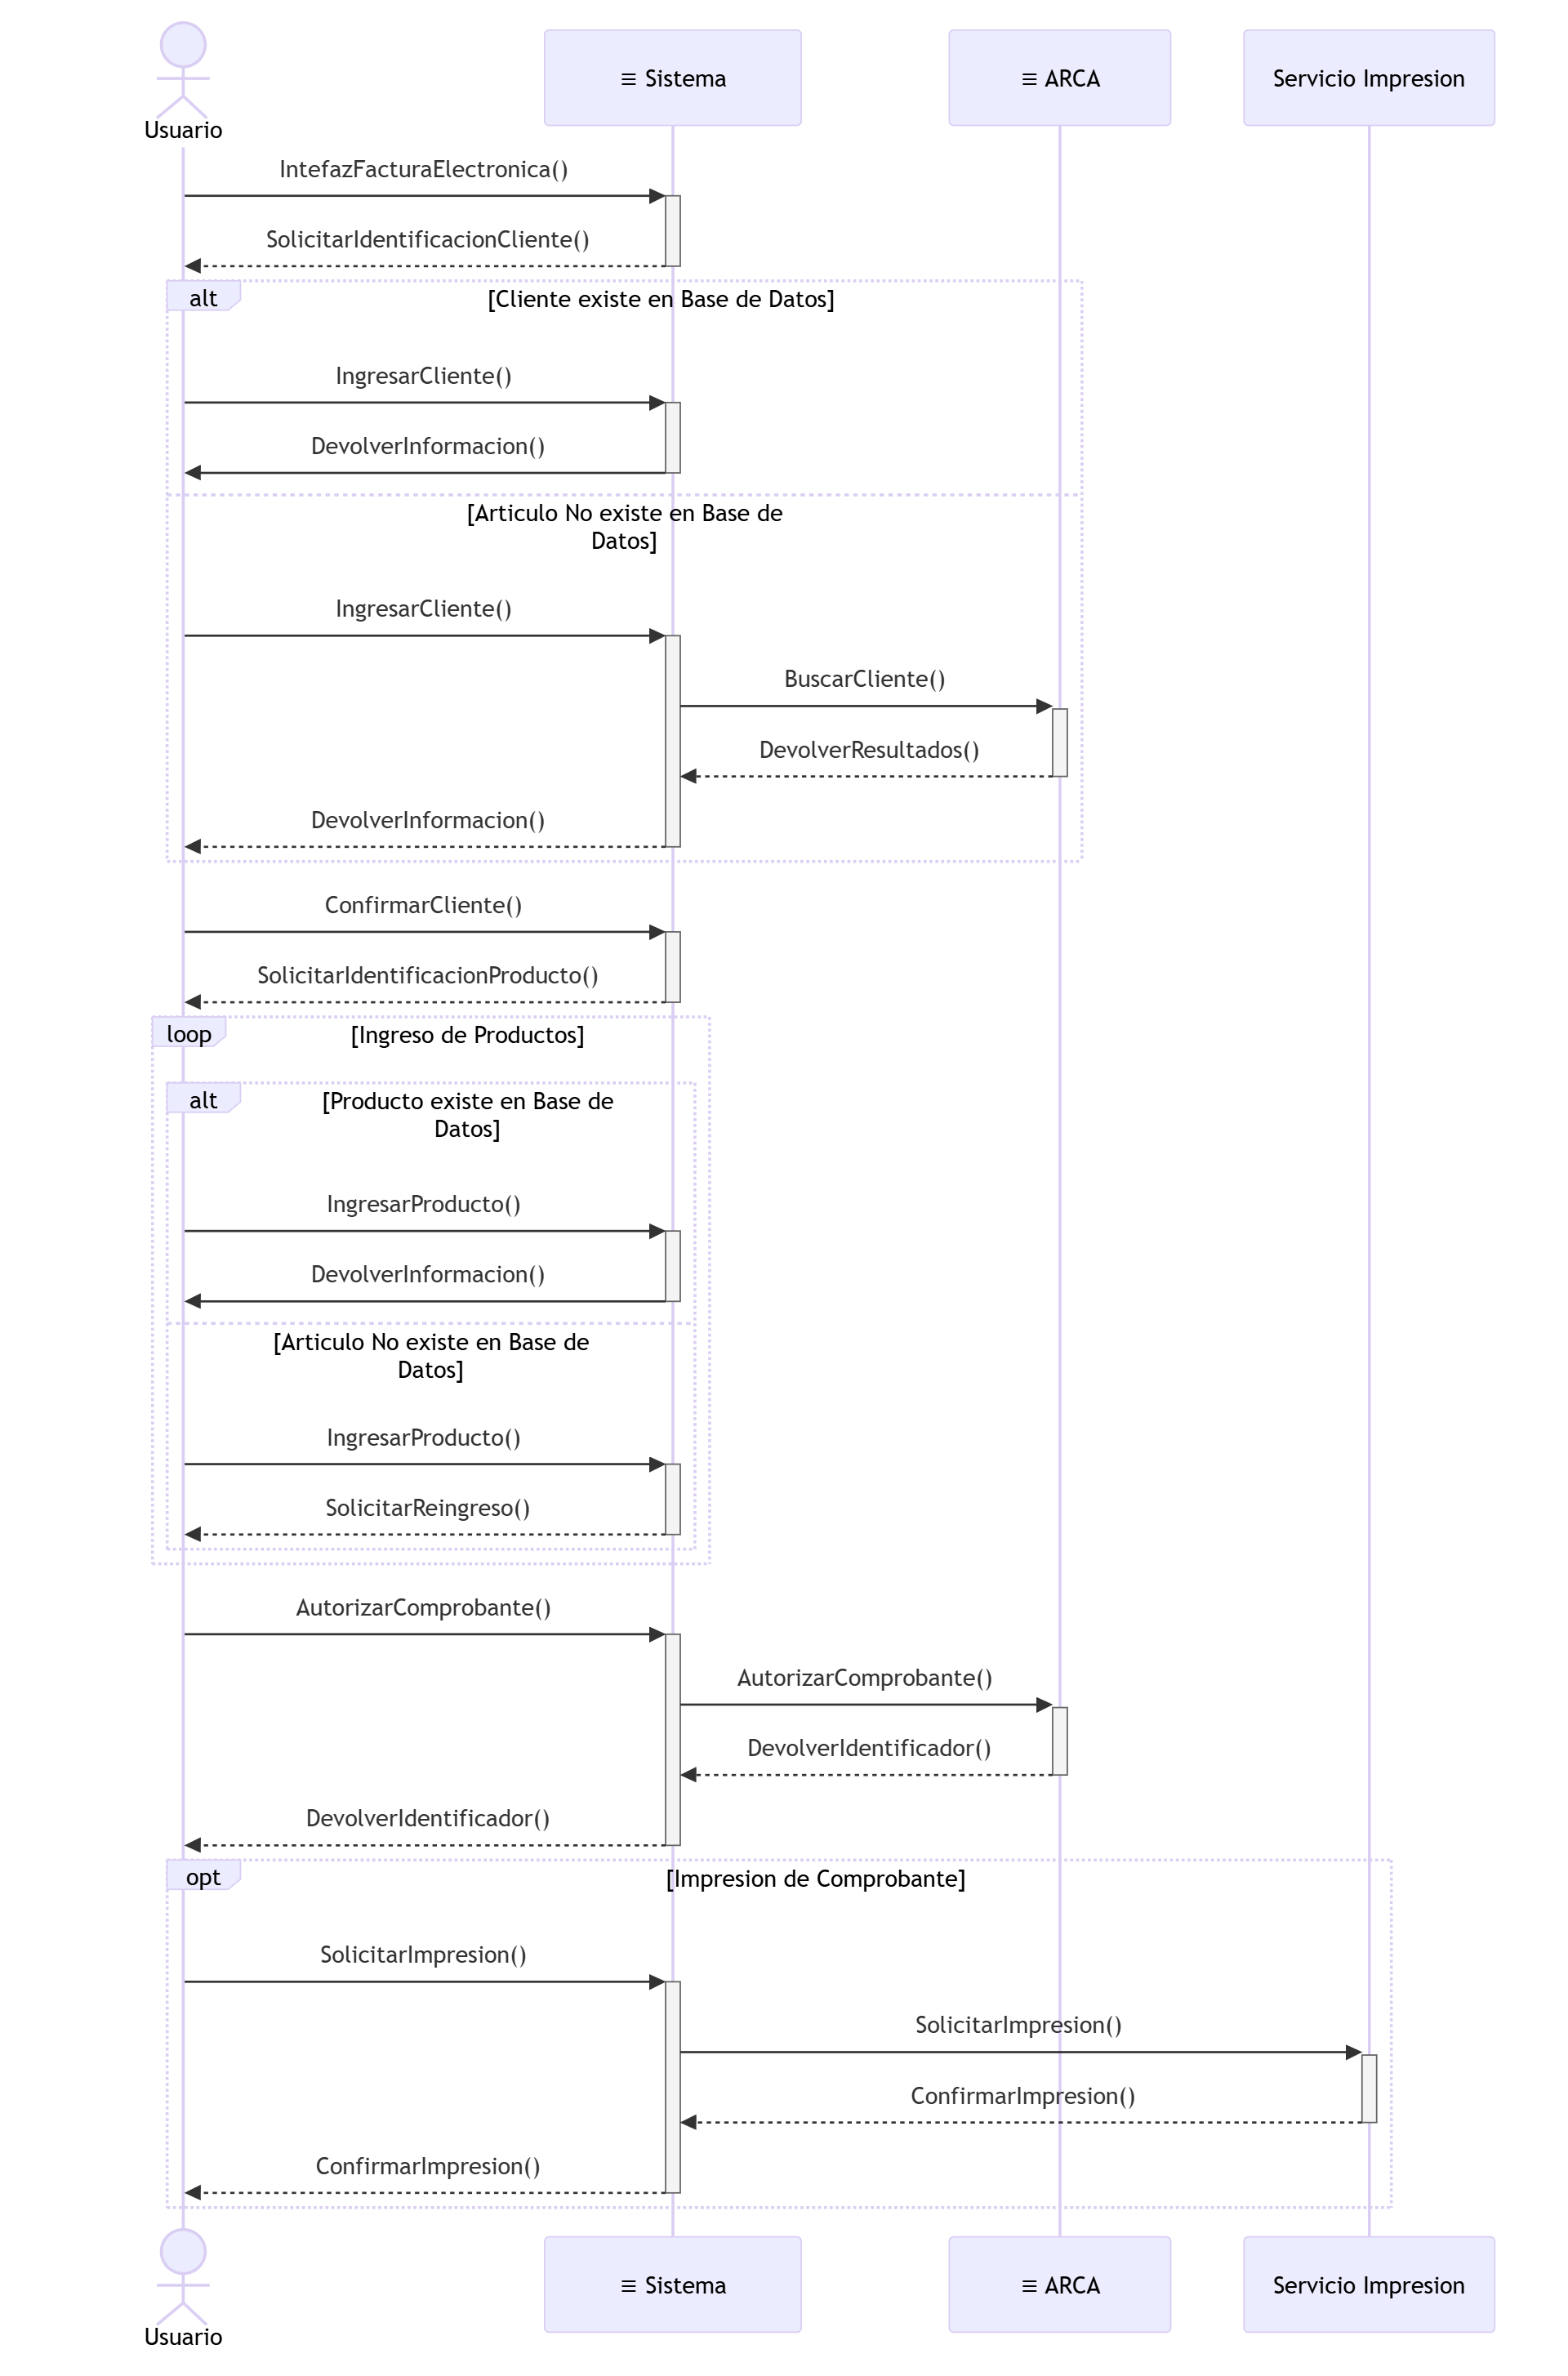
\includegraphics[width=.95\textwidth]{img/04-diagrama-caso-8.png}
	\vspace{15pt}
\end{figure}